\documentclass[letterpaper, reqno,11pt]{article}
\usepackage[margin=1.0in]{geometry}
\usepackage{color,latexsym,amsmath,amssymb,graphicx,float,listings,tikz}
\usepackage{hyperref}

\hypersetup{
colorlinks=true,
linkcolor=magenta,
filecolor=magenta,
urlcolor=cyan,
}

\tikzstyle{vertex}=[shape=circle, minimum size=2mm, fill, draw, inner sep=0]

\graphicspath{ {images/} }

\begin{document}
\pagenumbering{arabic}
\title{Math 443 Homework 7}
\date{22/03/23}
\author{Xander Naumenko}
\maketitle

{\medskip\noindent\bf Question 1.} Let $G$ be a $r$-regular graph that is not Eularian. By Euler's theorem, it must be that $r$ is odd, since otherwise it would be Eularian. The only way this is true is if
\[
||G| |=\frac{1}{2}\sum_{v\in G}d(v)=\frac{1}{2}|G| r
.\]
$r$ is odd and the left side is a whole number, so $|G|$ must be even. Since $G$ is regular $\overline{G}$ is also regular. Each of the vertices $v\in V(\overline{G})$ are connected to $\left(|G|-1\right)-r$. If this is zero then $\overline{G}$ is disconnected, otherwise $\left( |G|-1 \right) -r$ is even and each vertex in $\overline{G}$ has this degree, so by Euler's theorem $\overline{G}$ is Eularian. $\square$

{\medskip\noindent\bf Question 2.} Since $G_1$ and $\bar{G_1}$ are Eularian, using the same argument as in question 1, $|G|$ is odd and $|G|$ is even regular (i.e. it is $r$-regular with $r$ even). Since $G_2$ is non-Eularian, it must be that $G_2$ is odd regular, which again using the same argument as question 1 means that $|G_2|$ is even. This same argument applies identically for $G_3$. The total number of edges in $G$ will be the number of edges in each of $G_1,G_2,G_3$ plus the number of new edges added. This is:
\[
| |G| |=| |G_1| |+| |G_2| |+| |G_3| |+\left( |G_1| \right) \left( |G_2| \right) +\left( |G_2| \right) \left( |G_3| \right)+\left( |G_1| \right) \left( |G_3| \right)
.\]
All the terms above are even except for the $| |G_2| |$ and $| |G_3| |$ terms, so the sum is even. By Euler's theorem any graph with an even number of edges is Eularian, so $G$ is Eularian. $\square$

% {\medskip\noindent\bf Question 3.} The statement is true. Since $G$ is Eularian, there exists a sequence of edges $w=e_1\ldots e \ldots f \ldots e_n$ the forms a closed trail. Let $v$ be the shared vertex between $e$ and $f$. If $N(v)=\{e,f\} $, then $e$ and $f$ must already be adjacent in $w$ since the must enter/exit $v$ subsequently. Otherwise, separate $w$ into parts, each of which start and end on $v$. Since 

{\medskip\noindent\bf Question 3.} The statement is false. Consider the following graph: 

\begin{center}
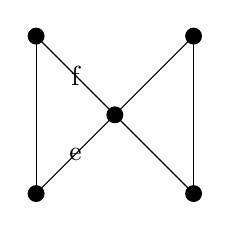
\begin{tikzpicture}
\draw (0,0)node[vertex]{};
\draw (0,2)node[vertex]{};
\draw (1,1)node[vertex]{};
\draw (2,0)node[vertex]{};
\draw (2,2)node[vertex]{};
\draw (0,0)--(0,2);
\draw (1,1)--(0,0)node[midway]{e};
\draw (1,1)--(0,2)node[midway]{f};
\draw (1,1)--(2,0);
\draw (1,1)--(2,2);
\draw (2,0)--(2,2);
\end{tikzpicture}
\end{center}

Clearly the graph is Eularian by traversing both triangles consecutively, starting from the middle vertex. To show that a closed trail can't use $e$ and $f$ consecutively, by way of contradiction assume there was a closed walk that contains $e$ and $f$ consecutively. Then part of the walk started and ended on the leftmost two vertices without visiting either of the rightmost vertices. However once this happens such a trail will never be able to get back to the rightmost vertices to make the trail Eularian, so such a trail can't exist and the above graph is a counterexample. $\square$

% {\medskip\noindent\bf Question 4.} Any multipartite complete graph with more than half of the vertices in one independent set can't be Hamiltonian, since any path can't have subsequent vertices in the same independent set. I claim that all other multipartite complete graphs are Hamiltonian. $\square$

% Let $G$ be a complete multipartite graph with $k$ maximal independent sets, none of which have more than $\frac{|G|}{2}$ vertices. Let $v$ be a vertex in a largest such set and add it to the end of a path $P$, then remove $v$ from $G$. Repeat this process repeatedly until all vertices are consumed. Note that this process will never terminate before $G$ is depleted, since we always choose the largest existing independent set to remove the next vertex from. This ensures that the number of vertices in the largest independent set is always less than or equal to half the existing vertices until the last vertex, so there will always be a choice available. Once this is finished $P$ is a spanning path, so $G$ is Hamiltonian. Thus the set of multipartite complete graphs that are Hamiltonian is the set of multipartite complete graphs with no independent set containing more than half of the vertices in the graph. $\square$

{\medskip\noindent\bf Question 5.} The statement is true. Let $S\subset V(G)$ be a set of vertices formed by taking one vertex from each component of $H$. Since they are taken from separate components of $H$, each element of $S$ is not adjacent in $G$, so $S$ is an independent set, which means $\alpha(G)\geq |S|$. We also have that $k(H)=|S|$, since we took one vertex from each component. Putting these together we get $k(H)\leq \alpha(G)$ as required. $\square$

{\medskip\noindent\bf Question 6.} As stated in the question the Petersen graph $G$ is non-Hamiltonian, so all we must prove is that for all $S\subset V(G)$, $k(G-S)\leq |S|$. Since $G$ has vertex connectivity $3$, $|S|=1$ and $|S|=2$ hold since in either case $k(G-S)=1\leq |S|$. Also using question 5, we know that $k(G-S)\leq \alpha((G)=4$, so the $|S|\geq 5$ cases are also handled. Thus either $|S|=3$ or $|S|=4$.

Consider removing the edges between the inside sections of the graph, i.e. separating $G$ into two copies of $C_5$, call this $G'$. We will prove that this subgraph of $G$ fulfills the property for $|S|\in \{3,4\} $, and since all we've done is remove edges it must also hold for $G$.

{\noindent\bf Case 1 ($|S|=3$):} If all three vertices in $S$ are in one of the cycles, then there are at most two components after the removal from that cycle, for a total $3\leq |S|$. If they are split two on one cycle and 1 from the other, then again the cycle with two vertices removed forms at most 2 components and the cycle with one vertex removed is still connected, for a total of $3\leq |S|$ components. By symmetry these are the only ways to split the vertices of $S$, so we're done. 

{\noindent\bf Case 2 ($|S|=4$):} If all 4 vertices of $S$ are in one cycle then clearly there are only $2\leq |S|$ components in $G'-S$. If it is split 3-1, there are up to two components resulting from the cycle with $3$ vertices removed and the other remains connected, for a total of $3\leq |S|$ components in $G'-S$. Finally if they are split 2-2 then each cycle has at most 2 components, for a total of $4\leq |S|$ components. Again by symmetry these are the only ways to split the vertices, so this case is finished. 

Since $G'-S$ has fewer than $|S|$ components, this also must hold for $G$ (since $k(G-S)\leq k(G'-S)$). We've covered all possible values of $|S|$, so the Petersen graph is a counterexample to the converse of Theorem 6.5. $\square$

{\medskip\noindent\bf Question 7.} Let $P_1$ be a Hamiltonian cycle in $G$, and let $G'=G-E(P_1)$. Since each vertex in $G$ had exactly two edges in $P_1$, we have that $\delta(G')=\delta(G)-2=\frac{|G|+4}{2}-2=\frac{|G|}{2}$. In class we proved that for any graph $G'$ with $\delta(G')\geq \frac{|G'|}{2}$, $G'$ is Hamiltonian. Let $P_2$ be a Hamiltonian path on $G'$. $P_1$ and $P_2$ are both Hamiltonian paths on $G$ and they are edge-disjoint by construction as required. $\square$

{\medskip\noindent\bf Question 8.} Consider a longest cycle $C$ in $G$. If $G=C$ then clearly $G$ is Hamiltonian by just removing any edge and taking the remaining path, so assume that $G\neq C$ as the only remaining case to consider. Then there exists a vertex $v\in V(C), u\in V(G)$ such that $uv\in E(G)$. Now consider the set of vertices containing $v, u$ and both neighbors of $v$ in $C$, call them $x$ and $y$. It can't be that both $ux\in E(G)$ and $uy\in E(G)$, since then $yCxuy$ would be a longer cycle, contradicting our assumption that $C$ is longest. Thus the subgraph induced by $\{x, y, u, v\} $ is isomorphic to either $K_{1,3}$ or $K_{1,3}+e$. However this was disbarred by the definition of $G$, so this case must have been impossible and $G$ is Hamiltonian. $\square$

{\medskip\noindent\bf Question 9.} Yes, the graph is Hamiltonian. See figure \ref{fig:q9} for a Hamiltonian cycle in $G$.

\begin{figure}[htpb]
    \centering
    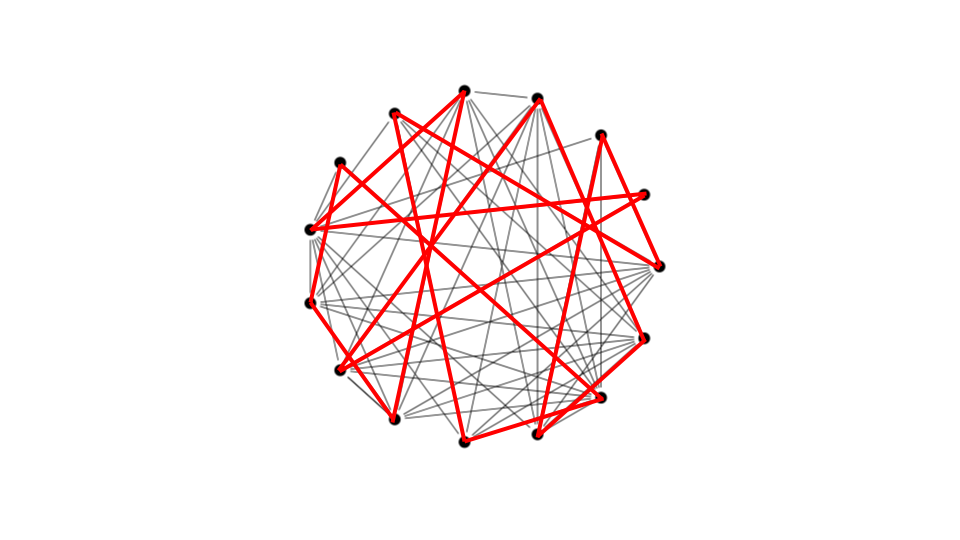
\includegraphics[width=0.8\textwidth]{q9}
    \caption{Hamiltonian cycle for question 9}
    \label{fig:q9}
\end{figure}

\end{document}
